%% use
%% library(cacheSweave)
%% Sweave("unmarked.Rnw", driver = cacheSweaveDriver)


\documentclass[article,shortnames]{jss}
\usepackage{amsmath,amssymb}
\usepackage[utf8]{inputenc}
\usepackage{rotating}
\usepackage{float}

\DeclareMathOperator{\logit}{logit}
\DeclareMathOperator{\Bern}{Bernoulli}
\DeclareMathOperator{\Bin}{Binomial}
\DeclareMathOperator{\Poi}{Poisson}
\DeclareMathOperator{\MN}{Multinomial}

\newcommand{\um}{\pkg{unmarked}}
\newcommand{\rlang}{\proglang{R}}
\newcommand{\scovs}{\code{siteCovs}}
\newcommand{\ocovs}{\code{obsCovs}}

\author{Ian J. Fiske\\North Carolina State University \And
  Richard Chandler\\ USGS Patuxent Wildlife Research Center}
\title{\pkg{unmarked}:\\
  An \proglang{R} package for the Analysis of Wildlife Occurrence and Abundance Data}

\Plainauthor{Ian Fiske, Richard Chandler}
\Plaintitle{unmarked: An R Package for the Analysis of Wildlife
  Occurrence and Abundance Data}
\Shorttitle{\um: Analyze Wildlife Data in \proglang{R}}

\Abstract{Ecological research uses data collection techniques that are prone 
to substantial and unique types of measurement error to address scientific 
questions about species abundance and distribution.  These data collection 
schemes include a number of survey methods in which unmarked individuals are 
counted, or determined to be present, at spatially-referenced sites.  
Examples include site occupancy sampling, repeated counts, distance sampling, 
removal sampling, and double observer sampling.  To appropriately analyze 
these data, hierarchical models have been developed to separately model 
explanatory variables of both a latent abundance or occurrence process and 
a conditional detection process.  Because these models have a straightforward 
interpretation paralleling mechanisms under which the data arose, they have 
recently gained immense popularity.  The common hierarchical structure of 
these models is well-suited for a unified modeling interface.  The 
\proglang{R} package \pkg{unmarked} provides such a unified modeling 
framework, including tools for data exploration, model fitting, model 
criticism, post-hoc analysis, and model comparison.}

\Keywords{ecological, wildlife, hierarchical, occupancy, occurrence, distance, point count}
\Plainkeywords{ecological, wildlife, hierarchical, occupancy, occurrence, distance, point count}


\Address{
Ian Fiske\\
Department of Statistics\\
North Carolina State University\\
2311 Stinson Drive \\
Campus Box 8203 \\
Raleigh, NC 27695-8203 \\
E-mail: \email{ijfiske@ncsu.edu}

Richard Chandler \\   
USGS Patuxent Wildlife Research Center \\
Gabrielson Lab, Room 226 \\
12100 Beech Forest Rd. \\
Laurel, MD 20708 \\
E-mail: \email{rchandler@usgs.gov} 
}



\usepackage{Sweave}
\begin{document}


\section{Introduction}


\subsection{Imperfect detection and data collection in ecological research}

A fundamental goal of ecological research is to understand how environmental 
variables influence spatial or temporal variation in species abundance or 
occurrence.  Addressing these research questions is complicated by imperfect 
detection of individuals or species.  Individuals may go 
undetected when present for a variety of reasons including their proximity to 
the observer, cryptic behavior, or camouflage. Thus, imperfect detection 
can introduce substantial measurement error and obscure underlying 
ecological relationships if ignored. 

To accommodate imperfect detection of individuals or species, 
ecologists have developed specialized methods to survey wildlife 
populations such as site occupancy sampling, repeated counts, 
distance sampling, removal sampling, and double observer sampling 
\citetext{see Section~\ref{sec:models-impl-unmark} and 
\citep{WilliamsEA2002} for definitions}.  This myriad of sampling methods 
are all unified by a common repeated-measures type of sampling design in 
which $J$ observations are made at $M$ spatial sample units during each of 
$T$ seasons. As an example, Table~\ref{tab:exdata} shows a typical 
repeated count dataset. 

\begin{table}[h] %\small
\begin{centering}
\begin{tabular}{lccccccc}
\hline
& \multicolumn{3}{c}{Season 1} && \multicolumn{3}{c}{Season 2} \\
\cline{2-4} \cline{6-8} 
        & Visit 1 & Visit 2 & Visit 3 && Visit 1 & Visit 2 & Visit 3 \\
\hline
Site 1  & 3       & 3       & 2       && 0       & 0       & 0 \\
Site 2  & 0       & 0       & 0       && 0       & 0       & 0 \\
Site 3  & 4       & 6       & 5       && 5       & 5       & 3 \\
Site 4  & 0       & 0       & 0       && 0       & 0       & 2 \\  
\hline
\end{tabular}
\caption{An example of the data structure required by \um's fitting functions. 
Counts of organisms were made at $M=4$ sites during $T=2$ seasons with $J=3$ 
visits per season.}
\end{centering}
\label{tab:exdata}
\end{table}

In addition to the repeated-measures design, there are two important 
features to note about the data shown in Table~\ref{tab:exdata}.  First, 
the counts are of individuals that cannot be uniquely recognized, so 
although it may be possible to determine if three individuals were detected 
on two different visits (as was the case at Site 1 in Table~\ref{tab:exdata}), 
it is not possible to determine if they were the {\it same} three 
individuals. Second, this design is often referred 
to as a `metapopulation design' because the population may be regarded as an
aggregation of subpopulations and because the spatial sampling is 
an explicit component of the problem. This is important because it provides 
a basis for modeling variation among sites as a function of site-specific 
covariates, and because metapopulation 
parameters such as local colonization and extinction can be directly estimated. 

Both the metapopulation design and absence of individual recognition 
distinguish these data from data collected using another large suite of 
ecological sampling methods known as `capture-recapture' methods. A vast number 
of models have been developed for capture-recapture data, and many of them 
are implemented in the software program \emph{MARK} 
\citep{whiteBurnham99_MARK}. The origins of \um\ (the package and its name) 
arose to fill the void of models for data from studies of unmarked 
individuals involving explicit spatial sampling. 

\subsection{Hierarchical Models for Metapopulation Designs}

While many ecological studies produce data consistent with a 
metapopulation design, the development and implementation of 
models for inference under individual sampling protocols has 
proceeded in a piecemeal fashion, without a coherent analysis 
platform. Recently, however, a broad 
class of hierarchical models \citetext{see \citet{royleDorazio08} for a 
general treatment} has been developed that offers a unified 
framework for analysis by formally recognizing that observations are 
generated by a combination of (1) a \emph{state} process 
determining abundance or species occurrence at each site and (2) a 
\emph{detection} process that yields observations conditional on the 
state process. The model for the state process describes abundance or 
occurrence at each site, but due to imperfect detection, these quantities 
cannot be observed directly and are regarded latent variables. 

This paper introduces \um, an \rlang\ package that provides a 
unified approach for fitting this broad class of hierarchical 
models developed for sampling biological populations.  Inference in \um\ 
is based on the integrated likelihood wherein the latent state 
variable is marginalized out of the conditional likelihood.


\subsection[Scope and features of unmarked]{Scope and features of \pkg{unmarked}} 

\um\ provides tools to assist researchers with every step of the analysis 
process, including data manipulation and exploration, model fitting, post-hoc 
analysis, model criticism, and model selection.  \um\ provides a growing list 
of model-fitting functions designed for specific 
sampling methods.  The fitting functions each find the maximum likelihood 
estimates of parameters from a particular model 
(Section~\ref{sec:fitting-models}) and return an object that can be easily 
manipulated.  Methods exist for performing numerous post-hoc analyses such as 
requesting linear combinations of parameters, back-transforming parameters to 
constrained scales, determining confidence intervals, and evaluating goodness 
of fit.  The model specification syntax of the fitting functions was designed 
to resemble the syntax of \rlang's common fitting functions such as \code{lm} 
for fitting linear models.

Although there is existing software for fitting some of these models 
\citetext{e.g. \citep{Hines2002}}, there are a number of advantages to a unified 
framework within \rlang.  Many researchers are already familiar with \rlang\ 
and use its powerful data manipulation and plotting capabilities.  Sometimes 
many species are analyzed in tandem, so that a common method of aggregating 
and post-processing of results is needed, a task easily accomplished in 
\rlang.  Unlike other available software, \um\ makes it possible to map 
habitat-specific abundance and species distributions when combined with 
\rlang's GIS capabilities.  Another important advantage of \um's approach is 
that researchers can simulate and analyze data within the same 
computational environment.  This work flow permits simulation studies for power 
analysis calculations or the effectiveness of future sampling designs.  All of 
this is made much simpler by analyzing the data within \rlang, and using a 
single environment to complete all phases of the analysis is much less 
error-prone than switching between applications. 

In this paper, Section~\ref{sec:models-impl-unmark} gives a brief summary of 
many of the models \um\ is capable of fitting.  
Section~\ref{sec:unmarked-usage} describes general \um\ usage aided by a 
running data example.

\section[Models implemented in unmarked]{Models implemented in \um}
\label{sec:models-impl-unmark}

The list of models implemented in \um\ continues to grow as new models are 
developed. Table~\ref{tab:models} shows the models available as of version 
0.9-0.  Rather than describe each fitting function in detail, this section 
provides a summary of several of the most common sampling techniques and how 
\um\ can be used to model the resulting data. 

\begin{table}[ht] \footnotesize
%\begin{sidewaystable} \small
%\begin{tabular}{lp{2cm}cc}
\begin{tabular}{lccc}
\hline
\textbf{Model} & \textbf{Fitting} & \textbf{Data} & \textbf{Citation} \\ 
               & \textbf{function}&& \\ \hline
Single-season Occupancy & \code{occu} & unmarkedFrameOccu & \citealt{MacKenzie2002} \\
Abundance from presence-absence & \code{occuRN}& unmarkedFrameOccu & \citealt{Royle2003} \\
Abundance from repeated counts &\code{pcount}& unmarkedFramePCount & \citealt{Royle2004} \\
Distance-sampling &\code{distsamp}& unmarkedFrameDS & \citealt{Royle2004b} \\
Multinomial Counts &\code{multinomPois}& unmarkedFrameMPois & \citealt{Royle2004a} \\
Repeated Multinomial Counts &\code{gmultmix} & unmarkedFrameGMM & \citealt{chandlerEAip_TempEm} \\
Multi-season Occupancy &\code{colext}& unmarkedMultFrame & \citealt{MacKenzie2003} \\
Multi-season Abundance & \code{pcountOpen} & unmarkedFramePCO & \citealt{DailMadsen2011} \\
\hline
\end{tabular}
\caption{Models currently handled by unmarked along with their associated
  fitting functions (Section~\ref{sec:models-impl-unmark}) and data
  type (Section~\ref{sec:data-requirements}).}
\label{tab:models}
%\end{sidewaystable}
\end{table}

\subsection{Site occupancy models}

\subsubsection{Single season site occupancy model} 
\label{sec:occ}
 
An important state variable in ecological research is species occurrence 
(or `site occupancy'), say $Z_{i}$, a binary state variable such that 
$Z_{i}=1$ if site $i$ is occupied by a species and $Z_{i}=0$ otherwise.
Much interest is focused on estimating functions of species occurrence 
(e.g., number of occupied sites) or to identify factors that are
associated with changes in the probability of a site being
occupied, i.e., $\psi_{i}  = \Pr(Z_{i}=1)$. To estimate these parameters, 
researchers employ a sampling design, whereby surveyors visit a sample of $M$
sites and record the binary response $Y_{ij}$ of species detection ($Y=1$) or
non-detection ($Y=0$) during $j=1,\ldots,J_{i}$ visits to the $i$th site 
during a `season' \citep{MacKenzie2002}.  
A key feature of species occurrence surveys is that false absences are 
possible, so that a species might go undetected ($Y_{ij} =0$) even if it is 
present ($Z_{i} = 1$). A set of parameters $p_{ij}$ accounts for this 
observation process, where $p_{ij}$ is the
probability of detecting the species at site $i$ during visit $j$
given that site $i$ is truly occupied.  That is, 
$p_{ij} = \Pr(Y_{ij} = 1|Z_{i} = 1)$.

The key assumptions made when modeling these data are that the occupancy 
state at a site remains constant throughout the season and repeated visits at
a site are independent.  The first assumption is commonly referred to as the
`population closure' assumption, meaning that no births, deaths, emigrations,
or immigrations occur during the season.  
Season, therefore, will generally refer to a very short time frame, such as 
a few months during a breeding season, or even a few minutes if repeated 
visits are made in quick succession.  Replicate samples (i.e., $J>1$) are 
necessary to obtain information about the detection rate separate from 
the occupancy rate.  

The following hierarchical model describes the joint distribution of the 
observations conditional on the latent occupancy state, and the marginal 
distribution of the latent occupancy state variable:
\begin{gather}
Z_i \sim \Bern(\psi_i) \text{\quad for $i=1,2,\dots,M$} \notag \\
Y_{ij}|Z_i \sim \Bern(Z_i p_{ij})\text{\quad for $j=1,2,\dots,J_{i}$} \notag
\end{gather}
Removing the latent $Z$ variables by marginalization yields the likelihood:

\begin{equation}
L(\psi, p | Y_{ij}) = 
 \prod_{i}^{M} \left\{
    \prod_{j}^{J} 
      \left(p^{Y_{ij}}(1-p)^{1-Y_{ij}}\right)
          \psi + I(Y_{i.}=0)(1-\psi) \right\},  
\end{equation}

where $I$ is the indicator function taking the value 1 if its argument is 
true, and 0 otherwise. The model and likelihood are easily generalizable to 
accommodate covariates on detection probability or occupancy.
Variables that are related to the occupancy state are modeled as

\begin{gather}
  \logit(\psi_i) = \mathbf x_i' \mathbf \beta, \notag
\end{gather}
where $\mathbf x_i$ is a vector of site-level covariates and $\mathbf \beta$
is a vector of their corresponding effect parameters.  Similarly, the
probability of detection can be modeled with
\begin{gather}
  \logit(p_{ij}) = \mathbf v_{ij}' \mathbf \alpha, \notag
\end{gather}
where $\mathbf v_{ij}$ is a vector of observation-level covariates and
$\mathbf \alpha$ is a vector of their corresponding effect parameters.  
Examples of site-level covariates include habitat characteristics such as 
vegetation height. Observation-level covariates could include time of day, 
date, wind speed, or other factors that might affect detection probability. 
The function \code{occu} implements this model.


\subsubsection{Multi-season site occupancy model} 

Sometimes the study objective is to understand the dynamics of the 
occupancy state over time. To obtain such information researchers conduct 
repeated occupancy studies (see Section~\ref{sec:occ}) at the same sample of 
sites over consecutive seasons \citep{MacKenzie2003} and seek to estimate
probabilities of colonization ($\gamma_{it}$) and extinction
($\epsilon_{it}$), where colonization is the change of an unoccupied
site to occupied and extinction if the change of an occupied site to
unoccupied.  If the occupancy status is assumed to evolve according to
a Markov process, then a 2-state finite hidden Markov model describes
these data.  Let $Y_{itj}$ denote the observed species occurrence
status at visit $j$ during season $t$ to site $i$.  Then
\begin{gather}
  Z_{i1} \sim \Bern(\psi_i) \notag \\
  Z_{it} \sim
  \begin{cases}
    \Bern(\gamma_{i(t-1)}) & \text{if $Z_{i(t-1)} = 0$} \notag \\
    \Bern(1-\epsilon_{i(t-1)}) & \text{if $Z_{i(t-1)} = 1$}
  \end{cases}, \\
  \text{for $t=2,3,\dots,T$} \notag \\
  Y_{itj} | Z_{it} \sim \Bern(Z_{it} p_{itj}) \notag
\end{gather}

This model generalizes the single season site occupancy model by relaxing the 
population closure assumption. To define the likelihood of this model, 
let $\phi_0 = (\psi, 1-\psi)$ and 

\begin{equation}
  \theta_{{\bf Y_{it}}} =
  \begin{pmatrix}
    \prod_{j}^{J} p I(Y_{ijt}=0)(1-p_{ijt}) \\
    I(\sum_{j}^{J} Y_{ijt}=0). \notag\\
  \end{pmatrix}
\end{equation}

Furthermore, let the matrix of one-step Markov transition probabilities be 

\begin{equation}
  \Phi_t =
  \begin{pmatrix}
    1-\epsilon & \epsilon \\
    1-\gamma & \gamma \notag\\
  \end{pmatrix}
\end{equation}

The likelihood is then

\begin{equation}
L(\psi,\epsilon,\gamma,p | Y_{ijt}) = 
 \prod_{i}^{M} \left\{
    \phi_0 \left\{ \prod_{t}^{T-1} \Phi_t \theta_{Y_{it}}  
        \right\} \theta_{Y_{iT}} \right\},
\end{equation}

which can be maximized by the \code{colext} function in \um. Again, 
each of the four model parameters $\psi$, $\gamma$, 
$\epsilon$, and $p$ can be modeled as functions of covariates on the logit 
scale. 


\subsection{Abundance models}

\subsubsection{Repeated count data}
\label{sec:repeated-count-data}

Occupancy is a crude summary of population structure and dynamics and, in 
practice, considerable effort is focused on obtaining information about 
abundance \citep{dorazio07}. A common sampling design for obtaining 
abundance information, 
analogous to the basic occupancy design described above, is to 
repeatedly visit a sample of $M$ sites $J$ times and
record the number of unique individuals observed at each site.
Similar assumptions are made as with occurrence data: (1) abundance at
a site remains constant during a season and (2) counts at a site are
independent.  \citet{Royle2004} presented the following hierarchical model for
repeated count data.  Let $N_i$ be the unobserved total number of
individuals using a site and define $Y_{ij}$ as the number of individuals 
observed during the $j$th visit.  Then,
\begin{gather}
\label{eq:pc2}
  N_i \sim f(\lambda_i, \theta) \text{\quad for $i=1,2,\dots,M$}  \notag\\
  Y_{ij}|N_{i} \sim \Bin(N_i, p_{ij})\text{\quad for $j=1,2,\dots,J_{i}$} \notag,
\end{gather}
where $\lambda_i$ is the abundance rate at site $i$ and $p_{ij}$ is
the detection probability during the $j$th visit to site $i$.  $f$ is
a discrete distribution with support restricted to $N_{i} \ge 0$ and
$\theta$ are extra parameters of $f$ other than the location
parameter, $\lambda_{i}$.  \um\ currently supports $f$ as Poisson or
negative binomial.  In the Poisson case, there is no $\theta$.  In the
negative binomial case, $\theta$ is a dispersion parameter, which is
useful when overdispersion is suspected.

As with the occupancy model, covariates may be included at either the
state (here, abundance) or detection levels, but abundance is modeled
through a log link to enforce it's positivity constraint.
\begin{gather}
  \log(\lambda_i) = \mathbf x_i' \mathbf \beta, \notag
\end{gather}
where $\mathbf x_i$ is a vector of site-level covariates and $\mathbf \beta$
is a vector of their corresponding effect parameters.  Similarly, the
probability of detection can be modeled with
\begin{gather}
  \logit(p_{ij}) = \mathbf v_{ij}' \mathbf \alpha, \notag
\end{gather}
where $\mathbf v_{ij}$ is a vector of observation-level covariates and
$\mathbf \alpha$ is a vector of their corresponding effect parameters.

The $N_{i}$ variables are latent and so analysis is carried out based on 
the integrated likelihood obtained by marginalizing each $N_{i}$ from the 
conditional likelihood \citep{Royle2004b}:

\begin{equation}
L(\lambda, p | Y_{ij}) = 
 \prod_{i}^{M} 
 \left\{ \sum_{N_{i}=max({\bf Y_i})}^{\infty}
          \left( \prod_{j}^{J} 
     \frac{N_{i!}}{ (N_{i}-Y_{ij})!} p^{Y_{ij}}(1-p)^{N_{i}-Y_{ij}} \right)
       \frac{e^{-\lambda} \lambda^N}{N!} \right\}.
\end{equation}

This likelihood can be maximized using the \code{pcount} function.  

The function \code{pcountOpen} implements a generalized form of this model
designed for `open' populations with temporaral dynamics governed by 
apparent survival and recruitment parameters \citep{DailMadsen2011}. Another
related model was described by \citet{Royle2003} and can be fit with the 
\code{occuRN} function. This model estimates abundance from site occupancy data  
by exploiting the link between abundance and detection probability. 
     
\subsubsection{General multinomial-Poisson mixture model}
\label{sec:gener-mult-poiss}
Here we discuss a more general class of models that can be customized by the
user for a variety of sampling methods, the multinomial-Poisson model
\citep{Royle2004a}.   The general form of this model is
\begin{gather}
\label{eq:mp2}
  N_i \sim \Poi(\lambda_i) \text{\quad for $i=1,2,\dots,M$}  \notag \\
  \begin{pmatrix}
    \mathbf Y_i\\
    N_{i} - \sum_{j=1}^{J} Y_{ij}
   \end{pmatrix}
  \bigg| N_{i} \sim \MN\left(N_i, 
  \begin{pmatrix}
    \boldsymbol \pi_i \\
    \pi_{i}^{*} 
  \end{pmatrix}\right) \notag
\end{gather}
where $N_i$ is the latent abundance at site $i$ as with the repeated
count model, and $\boldsymbol \pi_i=(\pi_{i1},\pi_{i2},\dots,\pi_{iJ})'$ is
the vector of cell probabilities of observing responses in the $J$
possible categories, and $\mathbf Y_{i}$ is the vector of counts
that were actually observed.  In general, $\boldsymbol \pi_i$ is
determined by the specific sampling method and
$\sum_{j} \pi_{ij} \le 1$ because detection is imperfect and
$\pi_{i}^{*}=1 - \sum_{j} \pi_{ij}$  is the probability of the species
escaping detection at site $i$.  

It is worth noting that the replication here is of a different 
nature -- not over time necessarily -- but still effectively replication as 
far as the design goes. That is, there are still repeated measurements at 
each site, but with a multinomial protocol, the replicate counts are 
{\it dependent} instead of independent. 

To illustrate the likelihood under a multinomial observation model, 
suppose that a sampling method produces a multinomial observation 
with 3 observable frequencies at each site. As before, $N_{i}$ are 
latent variables, and so inference is based on the integrated 
likelihood of ${\bf y}_{i}$ which is:

\begin{equation}
L(\lambda, p | {\bf Y}_i) = 
 \prod_{i=1}^{N} \left\{ 
  \sum_{N_{i}=\sum_{j}(Y_{ij})}^{\infty} \left(
 \frac{N_{i}!}{ Y_{i1}! Y_{i2}! Y_{i3}! Y_{i0}!}
  \pi_{1}^{Y_{i1}}
  \pi_{2}^{Y_{i2}}
  \pi_{3}^{Y_{i3}}
  \pi^{*N_{i}- Y_{i.}} \right)
 \frac{e^{-\lambda} \lambda^N}{N!} \right\}
\end{equation}
For this specific case of a multinomial-Poisson mixture, the likelihood 
simplifies analytically (to a product-Poisson likelihood).
The function \code{multinomPois} can be used to maximize this likelihood.

For multinomial-Poisson sampling methods, the actual observations are
an underlying categorical detection variable with $M \leq J$ levels so
that the $J$-dimensional $\mathbf Y_{i}$ is derived from the
$M$-dimensional raw counts in some sampling method-specific manner.
Thus, it is necessary to model the detection at the raw observation
level, denoted $p_{ik}$ for $k=1,2,\dots,M$ at site $i$.  Then we
derive the multinomial cell probabilities $\boldsymbol \pi_{i}$
through the sampling technique-specific relationship
$\pi_{ij}=g(p_{ik})$ where $p_{ik}$ is the underlying probability of
detection and $g$ is some sampling method-specific function.  

Thus, the only two requirements to adapt \um's general multinomial Poisson
modeling to a new sampling method is to specify $g$ and a binary 0-1
matrix that describes the mapping of elements of
$\mathbf p_{i} = (p_{i1},\dots,p_{iR})'$ to elements of
$\boldsymbol \pi_{i}$.  This mapping matrix, referred to in
\um\ as \code{obsToY}, is necessary to consistently clean
missing values from the data and relate observation-level covariates
with the responses.  The ($j$,$k$)th element of
\code{obsToY} is 1 only if $p_{ik}$ is involved in the computation of
$\pi_{ij}$.  The detection function $g$ is called \code{piFun} in \um.

Covariates may be included in either the
state (here, abundance) or detection models, through $\mathbf p_{i}$
(not $\boldsymbol \pi_{i}$).
\begin{gather}
  \log(\lambda_i) = \mathbf x_i' \mathbf \beta, \notag
\end{gather}
where $\mathbf x_i$ is a vector of site-level covariates and $\mathbf \beta$
is a vector of their corresponding effect parameters.  Similarly, the
probability of detection can be modeled with
\begin{gather}
  \logit(p_{ij}) = \mathbf v_{ij}' \mathbf \alpha, \notag
\end{gather}
where $\mathbf v_{ij}$ is a vector of observation-level covariates and
$\mathbf \alpha$ is a vector of their corresponding effect parameters.

We now describe two common sampling methods that can be modeled
with the multinomial-Poisson model: removal sampling and double
observer sampling.  These two methods are included in \um, but
additional methods may easily be specified by defining a user-specified 
\code{piFun} function and \code{obsToY} matrix.


\paragraph{Removal sampling }

Popular in fisheries, removal sampling is commonly implemented by 
visiting a sample of $M$ sites $J$ times each and trapping or 
otherwise capturing and then removing individuals at each visit.  Thus, 
$Y_{ij}$ is the number of individuals captured at the $j$th visit for 
$j=1,2,\dots,J$. We can specify $g$ for removal sampling as follows.  The
probability of an individual at site $i$ being captured on the first
visit is $\pi_{i1} = p_{i1}$.  The probability of capture on the $j$th
visit is
\begin{equation}
  \pi_{ij} = \prod_{k=1}^{j-1}(1 - p_{ik})p_{ij}, \notag
\end{equation}
for $j=2,\dots,J$ and the probability of not being sampled is
\begin{equation}
  \pi_{i,J+1} = 1 - \sum_{j=1}^{J}(\pi_{ij}) \notag
\end{equation}
Thus, the mapping matrix is an $J \times J$  matrix with ones in
the upper triangle,
\begin{equation}
  \begin{pmatrix}
    1 & 1 & \dots & 1 \\
    0 & 1 & \dots & 1 \\
    \vdots & & \ddots & \vdots \\
    0 & 0 & \dots  & 1 \notag
  \end{pmatrix}
\end{equation}


\paragraph{Double observer sampling}
\label{sec:double-observ-sampl}

Double observer sampling involves collecting data by a team of two surveyors
simultaneously visiting a site.  Each observer records a list of detected 
organisms, and at the end of the survey the two observers attempt to reconcile
their counts.  If individuals are not uniquely marked, this may be a difficult 
task in practice; however, assuming that individuals can be distinguised, the 
data at each site are a vector of length three $\mathbf Y_i$,
corresponding to the numbers of individuals seen by only observer one,
only observer two, and both observers.  Thus, for double observer sampling, 
$g$ is defined as follows.
\begin{equation}
  \mathbf \pi_i =
  \begin{pmatrix}
    p_{i1}(1-p_{i2}) \\
    (1-p_{i1})p_{i2} \\
    p_{i1}p_{i2} \\
    (1-p_{i1})(1-p_{i2}).
  \end{pmatrix} \notag
\end{equation}
The \code{obsToY} mapping matrix for double observer sampling is the
following $3 \times 2$ matrix.
\begin{equation}
  \begin{pmatrix}
    1 & 0 \\
    0 & 1 \\
    1 & 1 
  \end{pmatrix} \notag
\end{equation}

The flexibility of the \code{multinomPois} function has been extended even 
further in the \code{gmultmix} function to allow for a negative binomial
mixture {\citep{DorazioEA05} and to relax the population closure assumption
\citep{chandlerEAip_TempEm}. In addition, one of the most 
widely used sampling methods, known as distance sampling, yields data 
that can be modeled as a multinomial-Poisson mixture \citep{Royle2004b}.  In 
distance sampling, observers record the distance to organisms detected at 
$M$ sites on a single visit. The distance data are then binned into $J$ 
distance intervals and the multinomial cell probabilities are computed as 
a function of distance from the observer. Because distance sampling data 
are associated with many unique attributes such as distance interval 
ut-points and survey method (line-transect vs point count), we created 
the specialized function \code{distsamp} to fit the multinomial-Poisson model 
to distance sampling data.

\section[unmarked usage]{\pkg{unmarked} usage}
\label{sec:unmarked-usage}

\um\ provides data structures, fitting syntax, and post-processing that form a
cohesive framework for site-based ecological data analysis.  In order
to achieve these goals, \um\ uses the S4 class system
\citep{Chambers2008}. As \rlang's most modern system of class-based
programming, S4 allows customization of functions, referred to as
methods, to specific object classes and superclasses. For example,
when the generic \code{predict} method is called with any \um\ model
fit object as an argument, the actual \code{predict} implementation
depends on the specific model that was fit.  Use of class-based
programming can provide more reliable and maintainable software while
also making the program more user-friendly \citep{Chambers2008}.


\subsection{Preparing data}
\label{sec:data-requirements}

\um\ uses a custom S4 data structure called the \code{unmarkedFrame}
to store all data and metadata related to a sampling design.  Although this at
first appears to add an extra layer of work for the user, there are
several reasons for this design choice.  The multilevel structure of
the models means that standard rectangular data structures such as 
\code{data.frame}s or matrices are not suitable for storing the data.  For
example, covariates might have been measured separately at the site
level and at the visit level.  Furthermore, the length of the response
vector $\mathbf Y_{i}$ at site $i$ might differ from the number of
observations at the site as in the multinomial Poisson model.  In some 
cases, metadata of arbitrary dimensions may need to be associated with the 
data.  For example, in distance sampling it is necessary to store the units 
of measure and the survey design type.  Aside
from these technical reasons, \citet{Gentleman2009} pointed out that
the use of such portable custom data objects can simplify future
reference to previous analyses, an often neglected aspect of research.
Repeated fitting calls using the same set of data require less code
repetition if all data are contained in a single object.  Finally,
calls to fitting functions have a cleaner appearance with a more
obvious purpose when the call is not buried in data arguments.  The
parent data class is called an \code{unmarkedFrame} and each \um\
fitting function has its own data type that extends the
\code{unmarkedFrame}.  To ease data importing 
and conversion, \um\ includes several helper functions to automatically
convert data into an \code{unmarkedFrame}: \code{csvToUMF} which
imports data directly from a comma-separated value text file,
\code{formatWide} and \code{formatLong} which convert data from data
frames, and the family of unmarkedFrame constructor functions.

An \code{unmarkedFrame} object contains components referred to as slots, 
which hold the data and metadata. All \code{unmarkedFrame} objects contain 
a slot for the observation matrix \code{y}, a \code{data.frame} of 
site-level covariates \code{siteCovs}, and a \code{data.frame} of 
observation-level covariates \code{obsCovs}.  The \code{y} matrix is the 
only required unmarkedFrame slot. 
Each row of \code{y} contains either the observed counts or presence-absence
data at each of the $M$ sites.  \code{siteCovs} is an $M$-row \code{data.frame} 
with a column for each site-level covariate.  \code{obsCovs} is an $MJ$-row 
 \code{data.frame} with a column for each observation-level covariate.  Thus 
each row of \code{obsCovs} corresponds to a particular observation, with the 
order corresponding to site varying slower and observation within site
varying faster.  Both \scovs\ and \ocovs\ can contain \code{NA}
values corresponding to unbalanced or missing data.  If any terms in the model
specification are missing for that observation, \um\
automatically removes observations.  \um\ provides
constructor functions to make creating unmarkedFrames straightforward.
For each specific data type, specific types of unmarkedFrames extend
the basic \code{unmarkedFrame} to handle model-specific nuances.

\subsubsection{Importing repeated count data}

Here is an example of creating an \code{unmarkedFrame} for repeated count data
(Section~\ref{sec:repeated-count-data}). First, load the included data set of 
Mallard ({\it Anas platyrhynchos}) point counts described in \citet{Kery2005}.

\begin{Schunk}
\begin{Sinput}
> library(unmarked)
> data(mallard)
\end{Sinput}
\end{Schunk}

Loading the mallard data makes three objects available within the \rlang\ 
workspace. The matrix \code{mallard.y} contains the number of mallards counted
at each of $M=239$ sites (rows) on $J=3$ visits (columns).  The site-level 
covariates are columns of the \code{mallard.site} \code{data.frame}, 
which has $M$ rows. The observation-level covariates are a \code{list} 
with separate $M \times J$ matrices for each observation-level covariate.  
The unmarkedFrame constructors can accept \ocovs\ in this \code{list} format or 
as a \code{data.frame} in the format described in 
Section~\ref{sec:data-requirements}.

The following call to \code{unmarkedFramePCount} organizes the observations 
and covariates into an object that can be passed to the data argument of
the fitting function \code{pcount}.

\begin{Schunk}
\begin{Sinput}
> mallardUMF <- unmarkedFramePCount(y = mallard.y, siteCovs = mallard.site, 
+     obsCovs = mallard.obs)
\end{Sinput}
\end{Schunk}

Printing unmarkedFrames shows them as \code{data.frame}s to make it easier 
to verify that the data were converted correctly. Here only the first 
five sites (rows) and the first two visits are shown. 


\begin{Schunk}
\begin{Sinput}
> mallardUMF[1:5, 1:2]
\end{Sinput}
\begin{Soutput}
Data frame representation of unmarkedFrame object.
  y.1 y.2   elev length forest ivel.1 ivel.2 date.1 date.2
1   0   0 -1.173  0.801 -1.156 -0.506 -0.506 -1.761  0.310
2   0   0 -1.127  0.115 -0.501 -0.934 -0.991 -2.904 -1.047
3   3   2 -0.198 -0.479 -0.101 -1.136 -1.339 -1.690 -0.476
4   0   0 -0.105  0.315  0.008 -0.819 -0.927 -2.190 -0.690
5   3   0 -1.034 -1.102 -1.193  0.638  0.880 -1.833  0.167
\end{Soutput}
\end{Schunk}

The first three columns contain the count data. The site-level covariates are 
elevation (elev), transect length (length), 
and the proportion of forest covering the site (forest).  The two 
observation-level covariates are a measure of survey effort (ivel) and the date 
of the survey (date).  Note that these variables are standardized to 
mean of 0 and unit variance.  We can also check data contents with a 
quick summary.

\begin{Schunk}
\begin{Sinput}
> summary(mallardUMF)
\end{Sinput}
\begin{Soutput}
unmarkedFrame Object

239 sites
Maximum number of observations per site: 3 
Mean number of observations per site: 2.76 
Sites with at least one detection: 40 

Tabulation of y observations:
   0    1    2    3    4    7   10   12 <NA> 
 576   54   11    9    6    1    1    1   58 

Site-level covariates:
      elev               length              forest         
 Min.   :-1.436000   Min.   :-4.95e+00   Min.   :-1.265000  
 1st Qu.:-0.956500   1st Qu.:-5.63e-01   1st Qu.:-0.956000  
 Median :-0.198000   Median : 4.50e-02   Median :-0.065000  
 Mean   :-0.000046   Mean   :-2.93e-05   Mean   : 0.000067  
 3rd Qu.: 0.994000   3rd Qu.: 6.26e-01   3rd Qu.: 0.790000  
 Max.   : 2.434000   Max.   : 2.25e+00   Max.   : 2.299000  

Observation-level covariates:
      ivel                date          
 Min.   :-1.75e+00   Min.   :-2.90e+00  
 1st Qu.:-6.66e-01   1st Qu.:-1.12e+00  
 Median :-1.39e-01   Median :-1.19e-01  
 Mean   : 1.50e-05   Mean   : 7.26e-05  
 3rd Qu.: 5.49e-01   3rd Qu.: 1.31e+00  
 Max.   : 5.98e+00   Max.   : 3.81e+00  
 NA's   : 5.20e+01   NA's   : 4.20e+01  
\end{Soutput}
\end{Schunk}

The summary reveals that only 40 sites have at least one detection. The 
tabulation of y observations provides additional evidence of sparse counts, 
with no mallards being detected during 576 of the surveys. The 58 NA values 
correspond to missing data. 


\subsubsection{Importing removal sampling data}

To illustrate the slightly different syntax for removal sampling data example, 
we will import data from a removal survey of ovenbirds 
({\it Seiurus aurocapillus}) described by \citet{Royle2004a}.  The data consist 
of a list named \code{ovendata.list} with 
a matrix \code{data} containing the removal counts for 4 visits and a 
\code{data.frame} called \code{covariates} containing site-level covariates 
information.

\begin{Schunk}
\begin{Sinput}
> data(ovendata)
\end{Sinput}
\end{Schunk}

This loads a \code{list} named ovendata.list with components for the 
observed count data and covariates.  The only additional specification 
required when creating an \code{unmarkedFrame} for the multinomial-Poisson
model is to specify the particular type of data as either 
\code{removal}, \code{double}, or \code{userDefined}.

\begin{Schunk}
\begin{Sinput}
> ovenFrame <- unmarkedFrameMPois(ovendata.list$data, siteCovs = ovendata.list$covariates, 
+     type = "removal")
> head(ovenFrame, 5)
\end{Sinput}
\begin{Soutput}
Data frame representation of unmarkedFrame object.
  y.1 y.2 y.3 y.4   site   ufp  trba
1   0   0   0   0 CAT003 23.43  62.5
2   1   0   0   0 CAT004 15.62  70.0
3   0   0   0   0 CAT011 35.54  90.0
4   0   0   0   0 CAT013 25.78  60.0
5   0   0   0   0 CAT017 25.00 122.5
\end{Soutput}
\end{Schunk}

\subsubsection{Preparing multi-season occupancy data}

The data structures are more complex when surveys were conducted over more 
than one season. The following toy examples demonstrates how to prepare data
for the \code{colext} fitting function if there were only four sites, two
visits per season, and three seasons.

\begin{Schunk}
\begin{Sinput}
> M <- 4
> J <- 2
> T <- 3
> y <- matrix(0:1, nrow = M, ncol = J * T)
> rownames(y) <- paste("site", 1:M, sep = "")
> cn <- paste("season", rep(1:2, each = 3), sep = "")
> cn <- paste(cn, paste("v", rep(1:3, 2), sep = ""), sep = "")
> colnames(y) <- cn
> y
\end{Sinput}
\begin{Soutput}
      season1v1 season1v2 season1v3 season2v1 season2v2 season2v3
site1         0         0         0         0         0         0
site2         1         1         1         1         1         1
site3         0         0         0         0         0         0
site4         1         1         1         1         1         1
\end{Soutput}
\begin{Sinput}
> umf <- unmarkedMultFrame(y = y, numPrimary = T)
\end{Sinput}
\end{Schunk}

The function \code{unmarkedMultFrame} accepts \scovs\ and \ocovs\ like all 
other unmarkedFrame classes, and it also has an argument \code{yearlySiteCovs}
that can accept a list of $M \times T$ \code{data.frame}s containing 
season-level covariates. The \code{numPrimary} argument specifies the 
number of seasons.

\subsection{Manipulating unmarkedFrames}
\label{sec:manip}

The various components of \code{unmarkedFrames} can be extracted and 
subsetted in a manner similar to the methods used to manipulate standard 
\rlang\ objects.  Subsetting can be accomplished using the `bracket' 
notation. For example, the first five rows of data and all three 
removal occasions can be extracted from the ovenbird removal study using

\begin{Schunk}
\begin{Sinput}
> ovenFrame[1:5, 1:3]
\end{Sinput}
\begin{Soutput}
Data frame representation of unmarkedFrame object.
  y.1 y.2 y.3   site   ufp  trba
1   0   0   0 CAT003 23.43  62.5
2   1   0   0 CAT004 15.62  70.0
3   0   0   0 CAT011 35.54  90.0
4   0   0   0 CAT013 25.78  60.0
5   0   0   0 CAT017 25.00 122.5
\end{Soutput}
\end{Schunk}

In some cases, the covariate data may need to be manipulated after the 
\code{unmarkedFrame} has been created. The following code demonstrates 
how to extract the site-level covariates, standardize those that are 
continuous (columns 2 and 3), and reinsert them back into the 
\code{unmarkedFrame}.

\begin{Schunk}
\begin{Sinput}
> sc <- siteCovs(ovenFrame)
> sc[, 2:3] <- scale(sc[, 2:3])
> siteCovs(ovenFrame) <- sc
\end{Sinput}
\end{Schunk}



\subsection{Fitting models}
\label{sec:fitting-models}

As introduced in Section~\ref{sec:models-impl-unmark}, each type of 
survey design 
has a corresponding fitting function.  For example, to fit a repeated count
model, we call \code{pcount}.  Table~\ref{tab:models} provides a
summary of all models that \um\ currently fits.  With the exception of the 
`open' population models (\code{colext}, \code{gmultmix}, and 
\code{pcountOpen}), all fitting functions use a double right-hand sided 
formula syntax representing the hierarchical model structure.  
Specifically, covariates affecting the detection process are specified 
following the first tilde, and covariates of the state process follow the 
second tilde. No left-hand side of the formula is specified because the 
unmarkedFrame defines the response variable uniquely as the \code{y} slot.

\subsubsection{Fitting a repeated count model}

Continuing the Mallard example, the following call to \code{pcount} fits a 
binomaial-Poisson mixture model (Section~\ref{sec:repeated-count-data}).  The 
following code specifies that detection probability $p$ should be modeled by 
day of year, including a quadratic term.  We also wish to model abundance 
using elevation and proportion of area forested.  As described in 
Section~\ref{sec:repeated-count-data}, covariates of detection are on the 
logit-scale and covariates of abundance are on the log scale for the 
repeated count model.

\begin{Schunk}
\begin{Sinput}
> fm.mallard.1 <- pcount(~date + I(date^2) ~ elev + forest, 
+     data = mallardUMF, K = 50)
> fm.mallard.1
\end{Sinput}
\begin{Soutput}
Call:
pcount(formula = ~date + I(date^2) ~ elev + forest, data = mallardUMF, 
    K = 50)

Abundance:
            Estimate    SE     z  P(>|z|)
(Intercept)   -1.853 0.236 -7.87 3.62e-15
elev          -1.232 0.234 -5.27 1.36e-07
forest        -0.756 0.165 -4.60 4.32e-06

Detection:
            Estimate     SE       z P(>|z|)
(Intercept)   0.3071 0.2149  1.4290 0.15301
date         -0.4091 0.1482 -2.7612 0.00576
I(date^2)    -0.0077 0.0853 -0.0903 0.92801

AIC: 521.2 
\end{Soutput}
\end{Schunk}

This initial fit suggests that Mallard abundance decreases with
increasing elevation and forest.  It also looks like a linear model
might suffice for the detection model, so we subsequently fit the
linear detection model as follows:


\begin{Schunk}
\begin{Sinput}
> fm.mallard.2 <- pcount(~date ~ elev + forest, data = mallardUMF, 
+     K = 50)
> fm.mallard.2
\end{Sinput}
\begin{Soutput}
Call:
pcount(formula = ~date ~ elev + forest, data = mallardUMF, K = 50)

Abundance:
            Estimate    SE     z  P(>|z|)
(Intercept)   -1.857 0.232 -7.99 1.37e-15
elev          -1.236 0.230 -5.38 7.59e-08
forest        -0.756 0.164 -4.60 4.23e-06

Detection:
            Estimate    SE     z  P(>|z|)
(Intercept)    0.298 0.188  1.58 0.113983
date          -0.401 0.114 -3.51 0.000449

AIC: 519.21 
\end{Soutput}
\end{Schunk}

This seems to be a better model according to both the Wald p-value and
AIC.  The result suggests that detection probability decreases during the 
course of a year.



\subsubsection{Fitting a multinomial-Poisson model}

Here we demonstrate fitting a multinomial-Poisson mixture model to removal 
sampling data.  The Ovenbird data has no observation-level covariates, so 
detection probability is assumed constant across visits.  It is not necessary
to specify that removal sampling was used when fitting the model
because this information is already stored in the \code{ovenFrame} data.
We model abundance as a function of understory forest coverage (\code{ufp})
and average basal tree area (\code{trba}).

\begin{Schunk}
\begin{Sinput}
> fm.oven.1 <- multinomPois(~1 ~ ufp + trba, ovenFrame)
> fm.oven.1
\end{Sinput}
\begin{Soutput}
Call:
multinomPois(formula = ~1 ~ ufp + trba, data = ovenFrame)

Abundance:
            Estimate    SE      z P(>|z|)
(Intercept)    0.102 0.119  0.864   0.388
ufp            0.100 0.126  0.794   0.427
trba          -0.171 0.135 -1.262   0.207

Detection:
 Estimate    SE    z P(>|z|)
    0.288 0.233 1.24   0.217

AIC: 326.14 
\end{Soutput}
\end{Schunk}


\subsection{Examining fitted models}
\label{sec:examining-model-fits}

Objects returned by \um's fitting functions also make use of the S4
class system.  All fitted model objects belong to the \code{unmarkedFit} 
parent class.  Thus, common operations such as extracting coefficient
estimates, covariance matrices for estimates, and confidence intervals
have been adapted to behave similar to \rlang's base functions.

For example, we can extract estimated coefficients either from the
entire model, or from the state or detection levels by specifying the
\code{type} argument.

\begin{Schunk}
\begin{Sinput}
> coef(fm.mallard.2)
\end{Sinput}
\begin{Soutput}
   lam(Int)   lam(elev) lam(forest)      p(Int)     p(date) 
   -1.85650    -1.23555    -0.75552     0.29776    -0.40061 
\end{Soutput}
\begin{Sinput}
> coef(fm.mallard.2, type = "state")
\end{Sinput}
\begin{Soutput}
   lam(Int)   lam(elev) lam(forest) 
   -1.85650    -1.23555    -0.75552 
\end{Soutput}
\end{Schunk}

To check which types are available for a model, use the \code{names} method.

\begin{Schunk}
\begin{Sinput}
> names(fm.mallard.2)
\end{Sinput}
\begin{Soutput}
[1] "state" "det"  
\end{Soutput}
\end{Schunk}

Similarly, the \code{vcov} function extracts the covariance matrix of
the estimates, using the observed Fisher information by default.

\begin{Schunk}
\begin{Sinput}
> vcov(fm.mallard.2, type = "det")
\end{Sinput}
\begin{Soutput}
           p(Int)   p(date)
p(Int)  0.0354902 0.0034485
p(date) 0.0034485 0.0130286
\end{Soutput}
\end{Schunk}

\code{vcov} also accepts a \code{type} argument, as does the convenience method 
\code{SE}, which returns standard errors from the square root of the diagonal 
of the covariance matrix. Extracting confidence intervals proceeds in a similar 
fashion.  By default, the asymptotic normal approximation is used.

\begin{Schunk}
\begin{Sinput}
> confint(fm.oven.1, type = "state", level = 0.95)
\end{Sinput}
\begin{Soutput}
                0.025   0.975
lambda(Int)  -0.12997 0.33471
lambda(ufp)  -0.14717 0.34776
lambda(trba) -0.43613 0.09441
\end{Soutput}
\end{Schunk}

Profile confidence intervals are also available upon request.  This
can take some time, however, because for each parameter, a nested
optimization within a root-finding algorithm is being used to find the
profile limit.

\begin{Schunk}
\begin{Sinput}
> ci <- confint(fm.oven.1, type = "state", level = 0.95, 
+     method = "profile")
\end{Sinput}
\begin{Soutput}
Profiling parameter 1 of 3 ... done.
Profiling parameter 2 of 3 ... done.
Profiling parameter 3 of 3 ... done.
\end{Soutput}
\end{Schunk}
\begin{Schunk}
\begin{Sinput}
> ci
\end{Sinput}
\begin{Soutput}
                0.025    0.975
lambda(Int)  -0.13908 0.326766
lambda(ufp)  -0.14777 0.348118
lambda(trba) -0.43684 0.094696
\end{Soutput}
\end{Schunk}

The profile confidence intervals and normal approximations are quite
similar here.

\subsubsection{The nonparametric bootstrap}

Nonparametric bootstrapping can also be used to estimate the
covariance matrix. \um\ implements a two-stage bootstrap in which the
 sites are first drawn with replacement, and then within each site, the
observations are drawn with replacement.  First, bootstrap draws must
be taken using the \code{nonparboot}.  \code{nonparboot} returns a new
version of the unmarkedFit object with additional bootstrap sampling
information.  Thus, this new fit must be stored, either in a new fit
object or the same one, and then subsequently queried for bootstrap
summaries.  In the following, bootstrapping can be quite slow.  For
these examples, we illustrate with the removal sampling data simply
because computations are much faster.  However, bootstrapping is
available for any of the models in \um.

\begin{Schunk}
\begin{Sinput}
> set.seed(1234)
> fm.oven.1 <- nonparboot(fm.oven.1, B = 10)
\end{Sinput}
\end{Schunk}

\begin{Schunk}
\begin{Sinput}
> SE(fm.oven.1, type = "state")
\end{Sinput}
\begin{Soutput}
 lambda(Int)  lambda(ufp) lambda(trba) 
     0.11854      0.12626      0.13534 
\end{Soutput}
\begin{Sinput}
> SE(fm.oven.1, type = "state", method = "nonparboot")
\end{Sinput}
\begin{Soutput}
 lambda(Int)  lambda(ufp) lambda(trba) 
     0.16400      0.14630      0.12881 
\end{Soutput}
\end{Schunk}

The bootstrapping and asymptotic standard errors are similar.

Additional bootstrap samples can be drawn by calling \code{nonparboot} again.
\begin{Schunk}
\begin{Sinput}
> fm.oven.1 <- nonparboot(fm.oven.1, B = 10)
\end{Sinput}
\end{Schunk}



\subsubsection{Linear combinations of estimates}

Often, meaningful hypotheses can be addressed by estimating linear
combinations of coefficient estimates.  Linear combinations of coefficient
estimates can be requested with \code{linearComb}.

Continuing the Ovenbird example, the following code estimates the
log-abundance rate for a site with \code{ufp = 0.5} and \code{trba
  = 0}.

\begin{Schunk}
\begin{Sinput}
> (lc <- linearComb(fm.oven.1, type = "state", coefficients = c(1, 
+     0.5, 0)))
\end{Sinput}
\begin{Soutput}
Linear combination(s) of Abundance estimate(s)

 Estimate    SE (Intercept) ufp trba
    0.153 0.130           1 0.5    0
\end{Soutput}
\end{Schunk}

Multiple sets of coefficients may be supplied as a matrix.  The
following code requests the estimated log-abundance for sites with
\code{ufp = 0.5} and \code{trba = 1}. 

\begin{Schunk}
\begin{Sinput}
> (lc <- linearComb(fm.oven.1, type = "state", coefficients = matrix(c(1, 
+     0.5, 0, 1, 1, 0), 2, 3, byrow = TRUE)))
\end{Sinput}
\begin{Soutput}
Linear combination(s) of Abundance estimate(s)

  Estimate    SE (Intercept) ufp trba
1    0.153 0.130           1 0.5    0
2    0.203 0.166           1 1.0    0
\end{Soutput}
\end{Schunk}

Standard errors and confidence intervals are also available for linear
combinations of parameters.  By requesting nonparametric bootstrapped
standard errors, \um\ uses the samples that were drawn earlier.

\begin{Schunk}
\begin{Sinput}
> SE(lc, method = "nonparboot")
\end{Sinput}
\begin{Soutput}
[1] 0.12882 0.13170
\end{Soutput}
\end{Schunk}

\subsubsection{Back-transforming linear combinations of coefficients}

Estimates of linear combination back-transformed to the native scale
are likely to be more interesting than the direct linear combinations.
For example, the logistic transformation is applied to estimates of
detection rates, resulting in a probability bound between 0 and
1. This is accomplished with the \code{backTransform}.  Standard
errors of back-transformed estimates are estimated using the delta
method.  Confidence intervals are estimated by back-transforming the
confidence interval of the original linear combination.

\begin{Schunk}
\begin{Sinput}
> (btlc <- backTransform(lc))
\end{Sinput}
\begin{Soutput}
Backtransformed linear combination(s) of Abundance estimate(s)

  Estimate    SE LinComb (Intercept) ufp trba
1     1.16 0.151   0.153           1 0.5    0
2     1.22 0.203   0.203           1 1.0    0

Transformation: exp 
\end{Soutput}
\begin{Sinput}
> SE(btlc)
\end{Sinput}
\begin{Soutput}
[1] 0.15101 0.20323
\end{Soutput}
\begin{Sinput}
> confint(btlc)
\end{Sinput}
\begin{Soutput}
    0.025  0.975
1 0.90339 1.5017
2 0.88463 1.6954
\end{Soutput}
\end{Schunk}

\subsection{Model selection} 

\pkg{unmarked} performs AIC-based model selection for structured lists of 
unmarkedFit objects.  To demonstrate, we fit a few more models to the Ovenbird
removal data, including an interaction model, two models with
single predictors, and a model with no predictors.

\begin{Schunk}
\begin{Sinput}
> fm.oven.2 <- update(fm.oven.1, formula = ~1 ~ ufp * trba)
> fm.oven.3 <- update(fm.oven.1, formula = ~1 ~ ufp)
> fm.oven.4 <- update(fm.oven.1, formula = ~1 ~ trba)
> fm.oven.5 <- update(fm.oven.1, formula = ~1 ~ 1)
\end{Sinput}
\end{Schunk}

Now, we can organize the fitted models with the \code{fitList} function and
the use the \code{modSel} method to rank the models by AIC.

\begin{Schunk}
\begin{Sinput}
> fmList <- fitList(`lam(ufp+trba)p(.)` = fm.oven.1, `lam(ufp*trba)p(.)` = fm.oven.2, 
+     `lam(ufp)p(.)` = fm.oven.3, `lam(trba)p(.)` = fm.oven.4, 
+     `lam(.)p(.)` = fm.oven.5)
> modSel(fmList)
\end{Sinput}
\begin{Soutput}
                  nPars    AIC delta AICwt cumltvWt
lam(trba)p(.)         3 324.77  0.00  0.35     0.35
lam(ufp)p(.)          3 325.73  0.96  0.21     0.56
lam(ufp+trba)p(.)     4 326.14  1.37  0.17     0.73
lam(.)p(.)            2 326.28  1.51  0.16     0.90
lam(ufp*trba)p(.)     5 327.17  2.40  0.10     1.00
\end{Soutput}
\end{Schunk}

It looks like the best model includes only tree basal area as a
predictor of abundance.  We can examine this relationship using
the \code{predict} method (Figure~\ref{fig:pred}).


\begin{figure}[ht]
  \centering
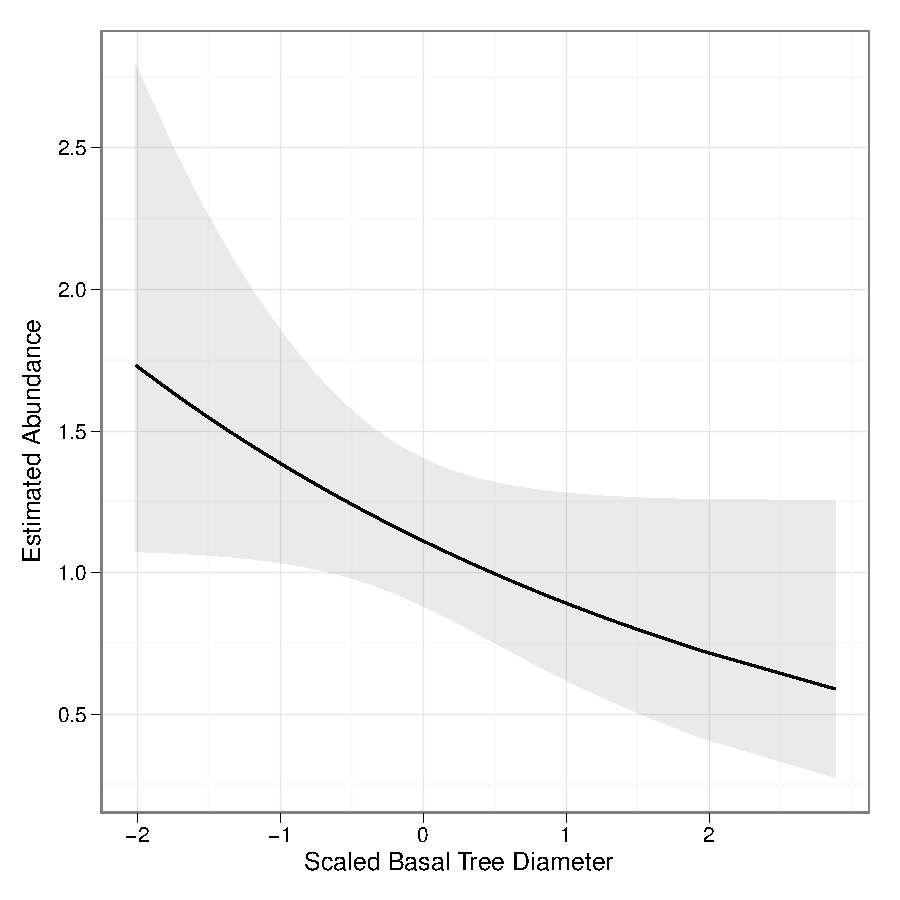
\includegraphics{unmarked-029}
\caption{Examine estimated abundance for Ovenbird removal data.  Band
  is 95\% confidence interval.}
\label{fig:pred}
\end{figure}

\begin{Schunk}
\begin{Sinput}
> preddata <- predict(fm.oven.4, type = "state", appendData = TRUE)
> library(ggplot2)
> qplot(trba, Predicted, data = preddata, geom = "line", 
+     xlab = "Scaled Basal Tree Area", ylab = "Estimated Abundance") + 
+     geom_ribbon(aes(x = trba, ymin = lower, ymax = upper), 
+         alpha = 0.1) + theme_bw()
\end{Sinput}
\end{Schunk}



\code{predict} functions much like \code{linearComb} except that new data can be
passed to it as a \code{data.frame} rather than a design matrix. When the first 
argument given to predict is a list of models created by \code{fitList}, 
\code{predict} computes model-averaged predictions, which may be
useful in the presence of high model selection uncertainty.  




\subsection{Goodness of fit and the parametric bootstrap}

To conduct goodness of fit tests, \um\ provides a generic parametric 
bootstrapping function.  It simulates data from the fitted model and 
applies a user-defined function that returns a fit-statistic such as the 
sum of squared residuals.  Beyond serving as a tool to evaluate goodness of fit,
\code{parboot} can be used to characterize uncertainty in any derived quantity 
of interest. Here we compute a chi-squared statistic to evaluate 
goodness of fit.

\begin{Schunk}
\begin{Sinput}
> set.seed(1234)
> chisq <- function(fm) {
+     observed <- getY(fm@data)
+     expected <- fitted(fm)
+     sum((observed - expected)^2/expected)
+ }
> pb <- parboot(fm.oven.1, statistic = chisq, nsim = 10)
\end{Sinput}
\end{Schunk}

\begin{Schunk}
\begin{Sinput}
> plot(pb, main = "")
\end{Sinput}
\end{Schunk}

\begin{figure}[hb]
  \centering
\includegraphics{unmarked-033}
\caption{Graphically assess model fit by parametric bootstrapping.  The dashed 
line is the observed chi-squared statistic. The histogram approximates the 
expected sampling distribution}
\label{fig:pb}
\end{figure}


The above call to \code{plot} with a parametric bootstrap object as
the argument produces a useful graphic for assessing goodness of fit
(Figure~\ref{fig:pb}).  The plot suggests that the model adequately  
explains these data.


\section[Future directions for unmarked development]{Future directions for \um\ development}
\label{sec:future-direct-unmark}

\um\ has become a stable and useful platform for the analysis of ecological 
data, but several areas of development could improve its utility.  First, new 
models need to be added to cover the range of sampling techniques and 
population dynamics commonly encountered. Table 3 illustrates the current 
gaps that need to be filled. In most cases, models to fill these gaps have not 
been developed so more research is needed.  


\begin{table}[h] \small
\begin{centering}
\begin{tabular}{lccc}
\hline
& \multicolumn{3}{c}{Population Dynamics} \\
\cline{2-4} 
Sampling method             & Closed              & Open to         & Open to \\
                            &                     & temporary       & demographic \\ 
                            &                     & emigration      & processess \\
\hline                            
Occurrence sampling         & \code{occu}         & ---             & \code{colext} \\
Repeated counts             & \code{pcount}       & ---             & \code{pcountOpen} \\
Removal sampling, \\double observer sampling,  & \code{multinomPois}& \code{gmultmix}  & --- \\
and other multinomial designs \\
Distance sampling           & \code{distsamp}     & ---               & --- \\
\hline
\end{tabular}
\caption{Model fitting functions classified by sampling method and population 
dynamics. Missing cells indicate models that have not been developed but are 
likely to be investigated in the future.} 
\label{tab:modelspace}
\end{centering}
\end{table}

Second, each of the models in \um\ assumes independence among sites. However, 
ecologists often use sampling methods such as cluster sampling that induce 
spatial dependence. Typically, this is done for logistical convenience, but 
because few methods are available to account for spatial correlation and 
imperfect detection probability, the spatial dependence is often ignored.  
Rather than this being a weakness of the sampling design, we envision that 
this dependence can be used as information regarding the spatial distribution
of individuals.  

Third, many of the likelihoods are written in pure \rlang, which can be 
slow for large problems. We are currently translating many of these
functions into \progland{C++} with the help of the R package \pkg{Rcpp} 
\citep{Rcpp11}.

Finally, Bayesian estimation could be implemented for many of these models.  An 
important advantage of Bayesian analysis over classical methods is that the 
latent abundance or occurrence variables can be treated as formal parameters.  
Thus posterior distributions could easily be calculated for derived parameters 
such as the proportion of sites occupied.  Bayesian analysis also would provide 
a natural framework for incorporating additional sources of random variation.  
For example, one could model heterogeneity among sites not accounted for by 
covariates alone.  

\section*{Acknowledgements}

The authors thank Andy Royle of the United States Geological Survey's
Patuxent Wildlife Research Center, who provided initial funding and
inspiration for this work.

%%\bibliographystyle{jss}
\bibliography{unmarked}

\end{document}
